\chapter{Exponentials and Logarithms}


Fold a sheet of paper in half, and it is twice as thick. Fold it again:
four times. If you could fold it 42 times, it would reach the Moon. That
is the power of repeated multiplication, and this chapter is about the
tools for handling it: exponents, and their opposites, logarithms. With
them, you can figure out when your savings will double, how long a glowing
watch keeps glowing, and how fast a video is going viral.

\section{Exponents}

Let us start with a quick review. Long ago, scientists noticed that their
formulas kept multiplying the same number by itself. For example, if they knew that a sphere was $r$
centimeters in radius, its volume in milliliters was

$$V = \frac{4}{3} \times \pi \times r \times r \times r$$

They did two things to make the notation less messy. First, they
decided that if two numbers were written next to each other, the
reader would assume that meant ``multiply them''. Second, they came
up with the exponent, a little number that was lifted off the
baseline of the text, that meant ``multiply it by itself''. For
example $5^3$ was the same as $5 \times 5 \times 5$.\index{exponents}

Now, the formula for the volume of a sphere is written

$$V = \frac{4}{3} \pi r^3$$

Tidy, right? In an exponent expression like this, we say that $r$ is
\index{exponents!base}\textit{the base} and $3$ is \index{exponent}\textit{the exponent}.

\subsection{Identities for Exponents}

What about exponents of exponents?  What is $\left(5^3\right)^2$?

$$\left(5^3\right)^2 = (5 \times 5 \times 5)^2 = (5 \times 5 \times 5)(5 \times 5 \times 5) = 5^6$$

In general, for any $a$, $b$, and $c$:

$$\left(a^b\right)^c = a^{(bc)}$$

If you have $\left( 5^3 \right) \left(5^4 \right)$, that is just $5 \times 5 \times 5 \times 5 \times 5 \times 5 \times 5$ or $5^7$

\index{exponents!product rule}The general rule is that for any $a$, $b$, and $c$

$$\left(a^b\right)\left(a^c\right) = a^{(b + c)}$$

Mathematicians \textit{love} this rule, so we keep extending the idea
of exponents to keep this rule true. For example, at some point,
someone asked ``What about $5^0$?'' According to the rule, $5^{2}$
must equal $5^{(2 + 0)}$ which must equal
$\left(5^2\right)\left(5^0\right)$.  Thus, $5^0$ must be 1. So
mathematicians declared ``Anything to the power of 0 is 1''.\index{exponents!zero}

We do not typically assume that $0^0 = 1$. It is just too
weird. So, we say that for any $a$ not equal to zero,

$$a^0 = 1$$

What about $5^{(-2)}$?  By our beloved rule, we know that
$\left(5^{-2}\right)\left(5^5\right)$ must be equal to $5^3$, right?
So $5^{-2}$ must be equal to $\frac{1}{5^2}$.\index{exponents!negative}

We say that for any $a$ not equal to zero and any $b$,

$$a^{-b} = \frac{1}{a^{b}}$$

This makes dividing one exponential expression by another (with the same base) easy:

$$\frac{a^b}{a^c} = a^{(b-c)}$$

We often say ``cancel out'' for this. Here, we can ``cancel out'' $x^2$:

$$\frac{x^5}{x^2} = x^3$$

What about $5^{\frac{1}{3}}$? By the beloved rule, we know that $5^{\frac{1}{3}}5^{\frac{1}{3}}5^{\frac{1}{3}}$ must equal $5^1$. \index{nth root}Thus, $5^{\frac{1}{3}} = \sqrt[3]{5}$.\index{exponents!fractions}

We say that for any positive $a$, any $b$, and any positive integer $c$,

\[
\large {a^{\frac{b}{c}}} = \left(\sqrt[c]{a}\right)^{b}=\left(\sqrt[c]{a^b}\right)
\]

Before you go on to the exercises, note that the beloved rule demands a common base.
\begin{itemize}
\item We can combine these: $\left(5^2\right)\left(5^4\right) = 5^6$
\item We cannot combine: $\left(5^2\right)\left(3^5\right)$
\end{itemize}

With that said, we note for any $a$,$b$, and $c$:

$$\left(ab\right)^c = \left(a^c\right) \left(b^c\right)$$

So, for example, if we were asked to simplify
$\left(3^4\right)\left(6^2\right)$, we would note that $6 = 2 \times
3$, so

$$\left(3^4\right)\left(6^2\right) = \left(3^4\right)\left(3^2\right)\left(2^2\right)  = \left(3^6\right)\left(2^2\right)$$


If these ideas are new to you (or maybe you are just having trouble remembering them),
watch the Khan Academy's \textbf{Intro to rational exponents} video at
\url{https://youtu.be/lZfXc4nHooo}.



\section{Logarithms}
After the world created exponents, it needed the opposite. We
could talk about the quantity $? = 2^3$, that is, ``What is the
product of 2 multiplied by itself three times?''  We needed some way
to talk about $2^? = 8$, that is, ``2 to the what is 8?'' This is why we
developed the logarithm.\index{logarithm} \index{log}

Here is an example:

$$\log_{2}8 = 3$$

In English, you would say, ``The logarithm base 2 of 8 is 3.''

The base (2, in this case) can be any positive number. The argument
(8, in this case) can also be any positive number.

Try this one: What is the logarithm base 2 of 1/16?

You know that $2^{-4} = \frac{1}{16}$, so $\log_{2} \frac{1}{16} = -4$.

\textbf{Worked example.} Find $\log_2 1024$ and $\log_{10} 0.001$.

\textbf{Solution.} $2^{10} = 1024$, so $\log_2 1024 = 10$. And
$10^{-3} = 0.001$, so $\log_{10} 0.001 = -3$. A logarithm just answers the
question ``what power?''

\begin{Exercise}[title={Solve for the Exponent}, label=exp1]
Solve $3^x = 81$. Then find $\log_5 125$ and $\log_4 2$.
\end{Exercise}
\begin{Answer}[ref=exp1]
$81 = 3^4$, so $x = 4$. Since $5^3 = 125$, $\log_5 125 = 3$. Since
$4^{1/2} = 2$, $\log_4 2 = \frac{1}{2}$.
\end{Answer}

\subsection{Logarithms in Python}

Most calculators have limited logarithm buttons, but
Python has a nice \pyfunction{log} function that lets you specify both
the argument and the base. Start python, import the math module, and try taking a few logarithms:\index{log!in python}

\begin{minted}{python}
>>> import math
>>> math.log(8,2)
3.0
>>> math.log(1/16, 2)
-4.0
\end{minted}

Say a friend offers you 5\% interest per year on your investment for as
long as you want. Each year, your money is multiplied by 1.05. You wonder, ``How many years
before my investment is 100 times as large?'' You can solve this problem with logarithms:

\begin{minted}{python}
>>> math.log(100, 1.05)
94.3872656381287
\end{minted}

If you leave your investment with your friend for 94.4 years, the
investment will be worth 100 times what you put in.

\subsection{Logarithm Identities}

The logarithm is defined this way:\index{logarithm!identities}

$$\log_b a = c \iff b^c = a$$

Notice that the logarithm of 1 is always zero, and $\log_b b = 1$.

\index{logarithm!product rule}The logarithm of a product:

$$\log_b a c = \log_b a + \log_b c$$

This follows from the exponent rule $b^{x + y} = b^x b^y$: logarithms
are exponents, so multiplying numbers adds their logarithms. What about a \index{logarithm!quotient rule}quotient?

$$\log_b \frac{a}{c} = \log_b a - \log_b c$$

Exponents?

$$\log_b \left(a^c\right) = c \log_b a$$

Notice that because logs and exponents are the opposite of each other, they can cancel each other out:

$$b^{\log_b a} = a$$

and

$$\log_b \left(b^a\right) = a$$

\subsection{Changing Bases}

We mentioned that most calculators have pretty limited logarithm
capabilities. Most calculators do not allow you to specify what base
you want to work with. All scientific calculators have a button for
``log base 10''.  So, you need to know how to use that button to get
logarithms for other bases. Here is the change-of-base identity:\index{logarithm!change of base}

$$\log_b a = \frac {\log_c a}{\log_c b}$$

For example, if you wanted to find $\log_2 8$, you would ask the
calculator for $\log_{10} 8$, then divide that by $\log_{10} 2$.
You should get 3.

\subsection{Natural Logarithm}

The circumference of a circle is about 3.141592653589793 times its
diameter.  Because we use
this unwieldy number a lot, we give it a name: We say ``The
circumference of a circle is $\pi$ times its diameter.''

There is a second unwieldy number that we will eventually use a great deal in
solving problems. It is about 2.718281828459045 (but the digits
actually go on forever, just like $\pi$). We call this number $e$. (You will see where $e$ comes from in the section on continuous compound
interest.)\index{e}\index{logarithm!natural}

Most calculators have a button labeled ``ln''. That is the
\textit{natural logarithm} button. It takes the log in base $e$.\index{ln}

Similarly, in python, if you do not specify a base, the logarithm is done in base $e$:

\begin{minted}{python}
>>> math.log(10)
2.302585092994046
>>> math.log(math.e)
1.0
\end{minted}

\subsection{Logarithms in Spreadsheets}

\index{logarithm!in spreadsheets}Spreadsheets have three log functions:
\begin{itemize}
\item \pyfunction{LOG} takes both the argument and the base. \pyfunction{LOG(8,2)} returns 3.
\item \pyfunction{LOG10} takes just the argument and uses 10 as the base.
\item \pyfunction{LN} takes just the argument and uses $e$ as the base.
\end{itemize}

Here is a plot from a spreadsheet of a graph of $y = LOG(x, 2)$.
\begin{figure}[H]
    \centering
    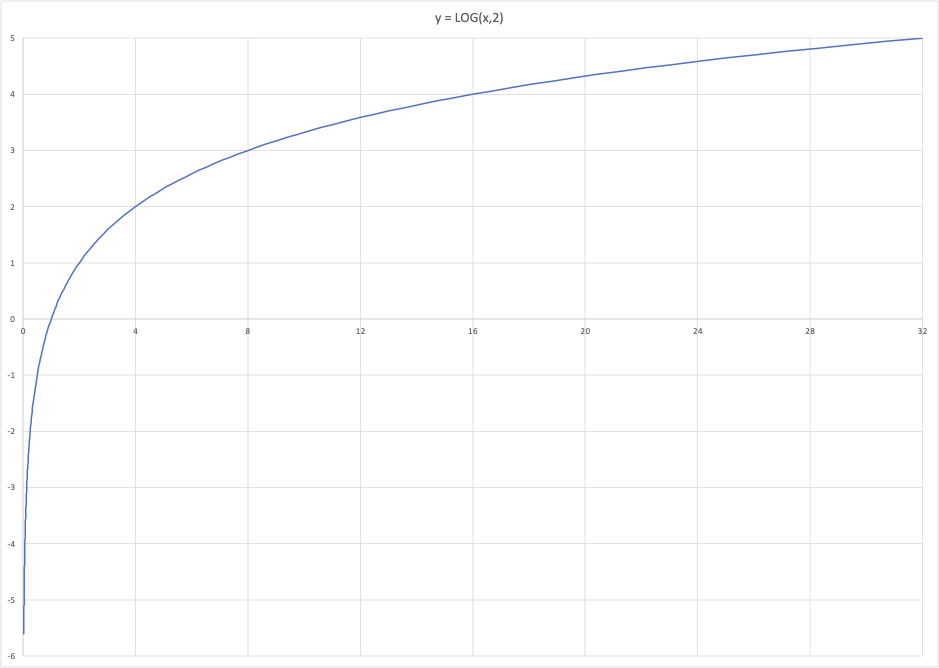
\includegraphics[width=0.8\textwidth]{log_graph.png}
    \caption{A graph of log base 2.}
    \label{fig:log_graph}
\end{figure}

Spreadsheets also have the \index{exponential function}function \pyfunction{EXP(x)}, which returns
$e^x$.  For example, \pyfunction{EXP(2)} returns 7.38905609893065.


\section{Compound Interest}
When you lend money, you usually charge interest. You may not think of it
this way, but a savings account is a loan: you lend your money to the
bank.  Any money you put in the account is loaned to
the bank. The bank then lends it to someone else, who pays interest to
the bank. The bank gives some of that interest to you.
% Diagram needed
However, what if you leave the interest in your account? And you start
making \textit{interest on the interest}? This is known as
\textit{compound interest}.\index{compound interest}

\subsection{An example with annual interest payments}

Let us say that you put \$1000 in a savings account that pays 6\%
interest every year. How much money would you have after 12 years?
Let us make a spreadsheet.

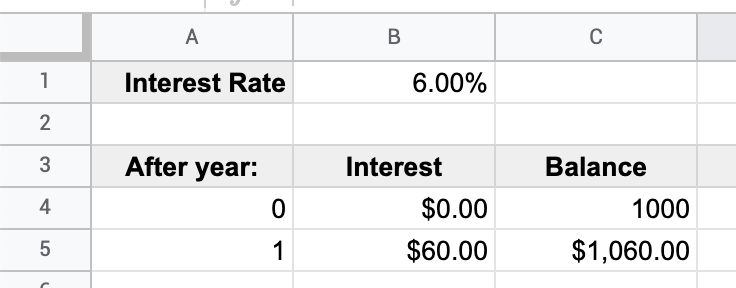
\includegraphics[width=0.4\textwidth]{StartInterest.png}

Create a new spreadsheet and edit the cells to look like this.  All
the cells in rows 1 - 4 are just values: just type in what you
see.

The fifth row is all formulas:

\begin{tabular}{c | c | c}
  After year & Interest & Balance \\
  \hline 
  = A4 + 1 & = B\$1 * C4 & = C4 + B5 \\
\end{tabular}

The interest rate field should be formatted as a percentage. One thing
to know when dealing with percentages in the spreadsheet: If the field
says ``600\%'', its value is 6. 

The cells in the Interest and Balance column should be formatted as currency.

You are about to make several copies of the cells in the fifth row,
so make sure they look right.

Click on A5 and shift-click on C5 to select all three cells. Drag the
lower-right corner down to fill the rows 6 - 15.

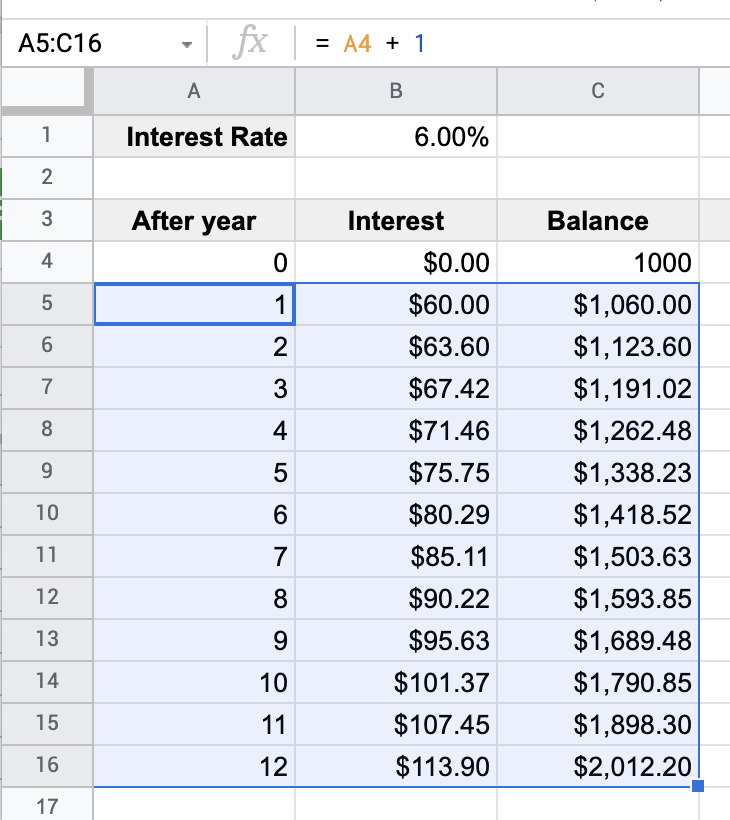
\includegraphics[width=0.5\textwidth]{CopiedCellsInterest.png}

Look at the numbers.  The first interest payment is \$60, but the last
is \$113.90. Your balance has more than doubled!

\subsection{Exponential Growth}

We figured this out numerically by repeatedly multiplying the balance
by the interest rate. What if you wanted to know what the balance
would be $n$ years after investing $P_0$ dollars with an annual interest
rate of $r$? (Note that $r$ in our example would be 0.06, not 6.0.)

Each year, the balance is multiplied by $1 + r$, so after one year,
$P_0$ would become $P_0 \times (1 + r)$.  The next year you would multiply
this number by $(1 + r)$ again: $P_0 \times (1 + r) \times (1 + r)$. The
next year? $P_0 \times (1 + r) \times (1 + r) \times (1 + r)$ See the
pattern? $P_n$ is this balance after $n$ years, then
\begin{equation}
  P_n = P_0 (1+r)^n
  \label{eq:compound}
\end{equation}

\ref{eq:compound} is referred to as the standard \newterm{compound interest formula}\index{compound interest formula}. 
Because $n$ is an exponent, we call this \textit{exponential growth}.
There are few things as terrifying to a scientist as
the phrase ``The population is undergoing exponential growth''.\index{exponential growth}

Many banks compound more often than once a year. If the bank compounds
$k$ times a year (12 for monthly, 365 for daily), it pays $\frac{r}{k}$
each time, and it does that $kt$ times in $t$ years. Your
\index{principal}principal $P_0$ grows to
$$P = P_0 \left(1+\frac{r}{k}\right)^{kt}$$

\subsection{Sensitivity to interest rate}

For most people, the first surprising thing about compound interest is
how quickly your money grows after a few years.  The second thing that
is surprising is how much difference a small change in the percentage
rate makes.

Let us add another set of columns that shows what happens to your money
if you convince the bank to pay you 8\% instead of 6\%.

Copy everything from columns B and C:

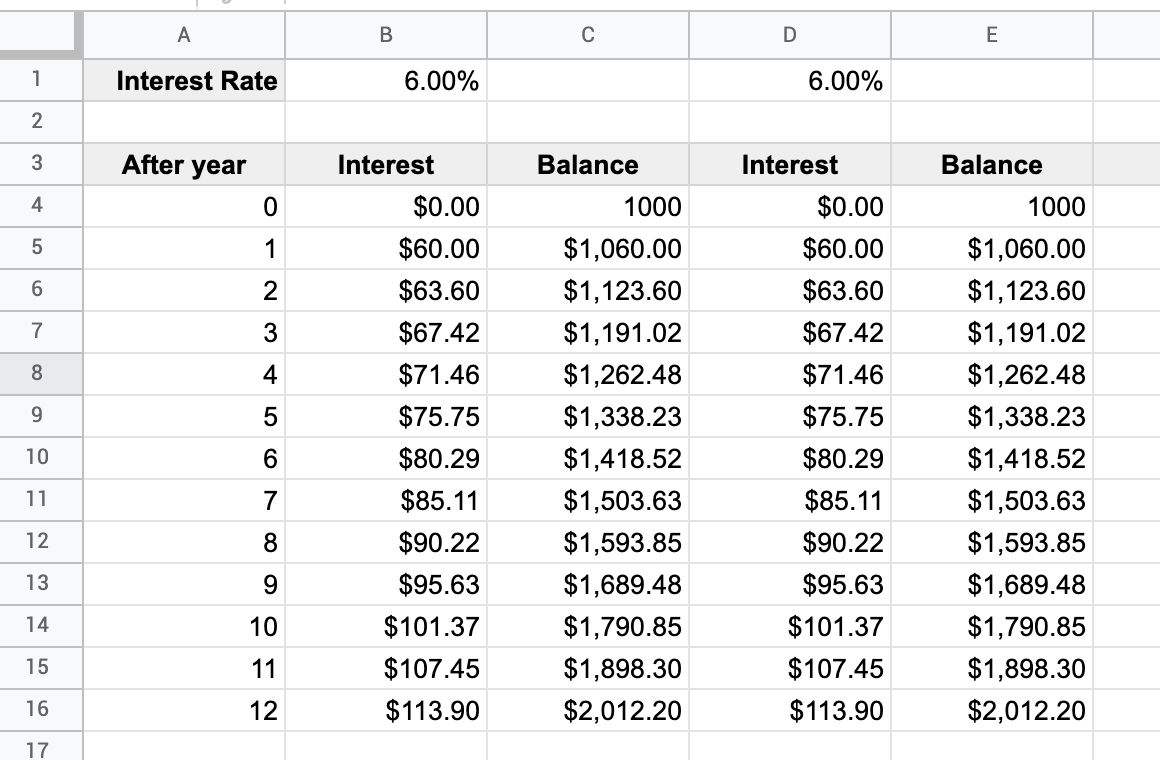
\includegraphics[width=0.6\textwidth]{CopyForSecondInterest.png}

Now edit the second interest rate to be 8\%:

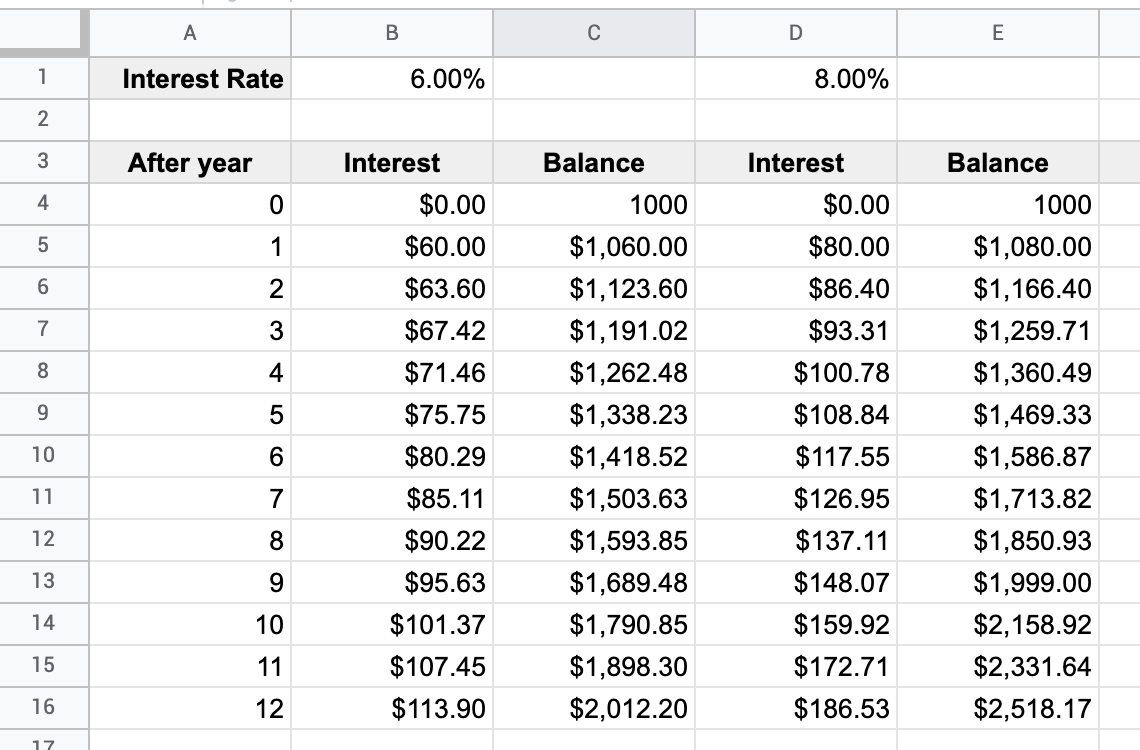
\includegraphics[width=0.6\textwidth]{AtBiggerInterestRate.png}

\subsection{Continuous Compound Interest}
Monthly beats yearly, and daily beats monthly. What if the bank compounded
every hour? Every second? Does your money grow without limit?

Try it with a 100\% interest rate for one year, starting with \$1. If the
bank compounds $k$ times, you end with $\left(1 + \frac{1}{k}\right)^k$
dollars:

\begin{center}
\begin{tabular}{l|r|l}
Compounding & $k$ & $\left(1 + \frac{1}{k}\right)^k$ \\
\hline
yearly & 1 & 2 \\
monthly & 12 & 2.613\ldots \\
daily & 365 & 2.7146\ldots \\
every second & 31{,}536{,}000 & 2.7182818\ldots
\end{tabular}
\end{center}

The answers creep up, but they never pass 2.71828\ldots. That number is
$e$! It is the most money \$1 can earn in a year at 100\% interest, no
matter how often the bank compounds. This is the real reason $e$ shows up
everywhere growth and decay happen.

With interest rate $r$ for $t$ years, compounding ``infinitely often''
gives the \index{continuous compounding}\newterm{continuous compound
interest} formula:
\begin{equation}\label{eq:continuous_compound}
  P = P_0e^{rt}
\end{equation}
(In the calculus volumes, you will learn to make ``infinitely often''
precise with a limit.)

\subsection{Practice Exercises}

\begin{Exercise}[label=compoundinterest1]
You deposit \$1500 into a savings account that pays an annual interest
rate of 5\%, compounded annually. What is the balance after 8 years?

Note: you can also use excel or google sheets built in function \texttt{=FV()}.
\end{Exercise}

\begin{Answer}[ref=compoundinterest1]
Using \ref{eq:compound} with $P_0 = 1500$, $r = 0.05$, and $n = 8$:
$$P_8 = 1500 (1+0.05)^8 = 1500 (1.05)^8 \approx \$2216.18$$

Alternatively, in Sheets/Excel, we can use \texttt{=FV(0.05, 8, 0, -1500)} to say that we want the \newterm{future value}\index{future value} of 1500 deposited (hence, negative), after 8 years compounded once per year.
\end{Answer}

\begin{Exercise}[label=compoundinterest2]
A bank offers two savings accounts, both with a stated annual interest
rate of 6\%. Account A compounds monthly ($k = 12$) and Account B
compounds daily ($k = 365$). If you deposit \$3000 into each account,
which account has the higher balance after 5 years, and by how much?

Create two columns in Excel/Sheets showing the balance after each year
for each account, using \$3000 as the principal. Start with year 0 for the
initial deposit, then fill in years 1 through 5 using the compound
interest formula for monthly and daily compounding.
\end{Exercise}

\begin{Answer}[ref=compoundinterest2]
Using $P = P_0 (1+\frac{r}{k})^{kt}$ with $P_0 = 3000$, $r = 0.06$, and $t = 5$ years:

Account A (monthly, $k=12$):
$$P = 3000 \left(1+\frac{0.06}{12}\right)^{12 \times 5} \approx \$4046.55$$

Account B (daily, $k=365$):
$$P = 3000 \left(1+\frac{0.06}{365}\right)^{365 \times 5} \approx \$4049.48$$

\begin{figure}[H]
    \centering
    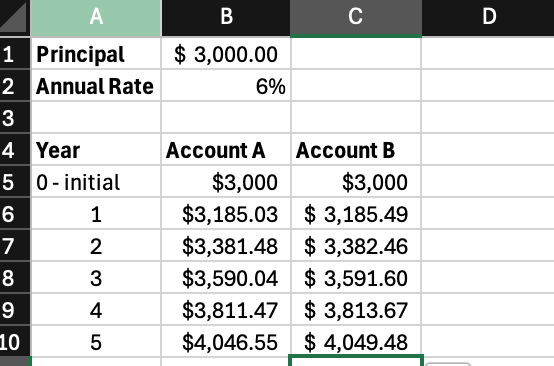
\includegraphics[width=0.8\textwidth]{exercise2sheet.png}
\end{figure}

Account B has the higher balance, by about \$2.93. This makes sense:
the more frequently interest is compounded, the closer the balance
gets to the continuous compounding limit, $P_0 e^{rt}$.
\end{Answer}

\section{Exponential Decay}
In the last section, an investment of $P$ earning
\index{compound interest}compound interest at an annual rate $r$ grew
exponentially. At the end of year $t$, the balance is

$$P\left(1 + r\right)^t$$

\index{exponential growth}Because $r$ is positive, this number grows as time passes. You get a
nice exponential growth curve that looks something like this:
\begin{figure}[H]
    \centering
    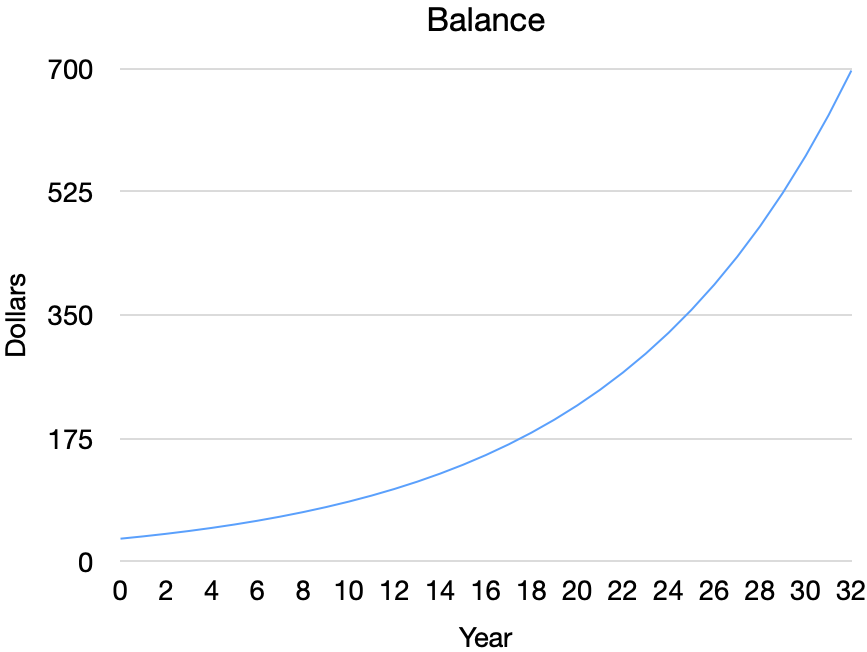
\includegraphics[width=0.7\textwidth]{exponential_growth.png}
    \caption{A diagram showing (exponential) compound interest.}
    \label{fig:exponential_growth}
\end{figure}

This is \$30 invested with a 10\% annual interest rate. So, the formula
for the balance after $t$ years would be

$$(30)(1.1)^t$$

What if $r$ were negative? This would be \textit{exponential decay}.

\subsection{Radioactive Decay}

Until around 1970, there were companies making watches whose faces and
hands were coated with radioactive paint. The paint usually contained
radium. When a radium atom decays, it gives off some energy, loses two
protons and two neutrons, and becomes a different element
(radon). Some of the energy given off is visible light. Thus, these
watches glow in the dark.\index{radioactive decay}

How many of the radium atoms in the paint decay each century? About 4.24\%.

Notice the quantity of atoms lost is proportional to the number of
atoms you have. This is exponential decay. If we assume that we start
with a million radium atoms, the number of atoms decreases over time like this:
\begin{figure}[H]
    \centering
    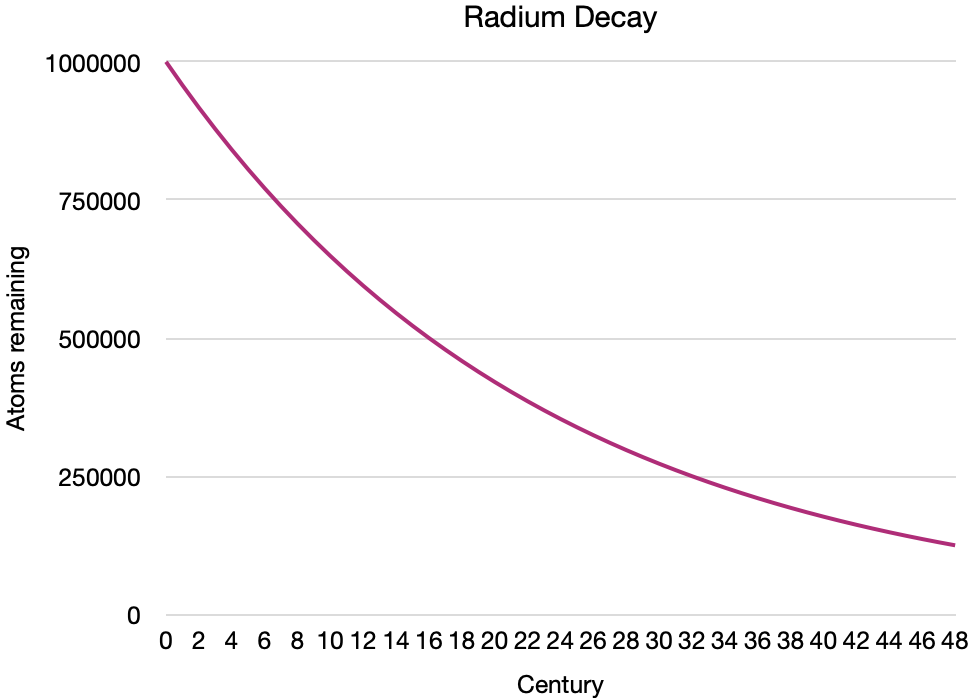
\includegraphics[width=0.7\textwidth]{radium_decay.png}
    \caption{A diagram showing the decay and half life of radium.}
    \label{fig:radium_decay}
\end{figure}
 
\begin{itemize}
\item We start with 1,000,000 atoms.
\item At 16 centuries, we have only 500,000 (half as many) left.
\item 16 centuries after that, we have only 250,000 (half again) left.
\item 16 centuries after that, we have only 125,000 (half again) left.
\end{itemize}

A nuclear chemist would say that radium has a \textit{half-life} of
1,600 years: every 1,600 years, half of whatever radium remains decays.
(Check: $(1 - 0.0424)^{16} \approx 0.50$.) This means that if you bought a watch with
glowing hands in 1960, it will be glowing half as brightly in the year
3560.\index{half-life}

How do we calculate the amount of radium left at the end of century
$t$? If you start with $P$ atoms, at the end of the $t$-th century, you
will have

$$P\left(1 - 0.0424\right)^t$$

This is exponential decay.\index{exponential decay}

\subsection{Model Exponential Decay}

\begin{Exercise}[title={A shrinking company}, label=exp_decay_company]
You are hired to run a company with 480,000 employees. Each year, $\frac{1}{8}$
of the employees leave (they retire, quit, or move away). For some reason,
you never hire anyone new.

Make a spreadsheet showing how many of the original 480,000 employees are
still around at the end of each of the next 12 years, and make a bar graph
of the data. Then write a formula for the number left after $t$ years, and
use logarithms to find when the company first drops below half its size.
\end{Exercise}
\begin{Answer}[ref=exp_decay_company]
Each year, $\frac{7}{8}$ of the employees stay, so after $t$ years there
are $480{,}000(0.875)^t$. The spreadsheet starts 480,000, 420,000, 367,500,
321,562, \ldots{} and ends with about 96,680 after 12 years.

Half the company is left when $(0.875)^t = 0.5$:
$$t = \frac{\log 0.5}{\log 0.875} \approx 5.19$$
So the company first drops below half its size during year 6 (after 6
years, 215,422 remain).
\end{Answer}


\definecolor{kontinuablue}{HTML}{005892}

Real data often curves. Populations grow exponentially, and radioactive
substances decay exponentially. You can force a line of best fit through
curved data, but it will be the wrong model. Logarithms can straighten
curves out, so you can use the line-fitting tools you already know.

Exponential growth and decay show up in data, too: video views, bacteria counts, and medicine in the
bloodstream. After you learn to fit straight lines to data, the Transforming Nonlinear Data with Logarithms
chapter shows how logarithms turn curves like these into straight lines that you can fit.
